% ----------------------------------------------------------
% Subseção Expansão binomial
% ----------------------------------------------------------
\subsection{Expansão binomial}
A lógica primordial (negação de si) cria expansões binomiais infinitas. O primeiro momento lógico é o início de uma dessas expansões, porém existem infinitas possibilidades de negação do primeiro momento lógico, o que revela as infinitas expansões binomiais. Uma expansão binomial é análoga a um universo. É importante observar que o primeiro momento lógico negar SER ilógico não transforma o ilógico em lógico, negar não é transformar. Essa é uma dualidade da lógica (SER ilógica e NÃO SER lógica) que garante as infinitas expansões binomiais, uma vez que o ilógico é imutável e por isso pode ser negado infinitamente.

\begin{quote}
"Em nossos dias vemos a expansão binomial de uma forma limpa e prática, sendo considerada um dos desenvolvimentos mais lindos e elegantes da matemática, vista com simplicidade em todos os níveis de ensino e pesquisa." \cite{ufpr_binomio_newton}.
\end{quote}
\begin{align*}
(x+a)^n &= \sum_{p=0}^{n}\binom{n}{p} a^p x^{n-p}
\end{align*}

\begin{figure}[H]
\caption{Momentos lógicos iniciais}
\label{fig:third_logical_moment}
\centering
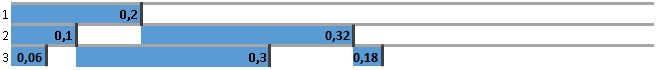
\includegraphics[scale=.85]{sections/images/third_logical_moment.jpg}
\floatfoot{Exemplo dos três primeiros momentos de uma expansão.}%\footnotemark}
\end{figure}
%\footnotetext{Fonte: note}

Com base na Figura \ref{fig:third_logical_moment} pode-se extrair as seguintes observações em relação ao primeiro, segundo e terceiro momentos lógicos:
\begin{description}
   \item[Primeiro momento lógico] A negação da lógica primordial a si, a subdivide em duas unidades, que somadas são o todo ilógico. Apesar dessas partes terem proporções diferentes, elas exprimem as mesmas quantidades de pontos ou possibilidades de mudança, uma vez que são representações da lógica primordial, que ad infinitum. A parte fracionada em azul representa a proporção da negação lógica em relação à sua unidade.
   \item[Segundo momento lógico] É gerado pela negação das duas sub-lógicas primordiais, fracionadas no primeiro momento lógico. Na impossibilidade dessas frações lógicas do primeiro momento lógico continuar negando a si, faria com que elas fossem incapazes de negar suas unidades que formam o todo, ou seja, seriam incapazes de negar as duas unidades e por consequência o todo que é formado precisamente por elas, o que faria da lógica apenas ilógica, uma unicidade. As partes fracionadas em azul representam a proporção da negação lógica em relação à sua respectiva unidade.
   \item[Terceiro momento lógico] Decorre da negação do segundo momento lógico, assim como o segundo momento lógico decorre da negação do primeiro e assim por diante.
\end{description}

A cada negação ou subnegação da lógica primordial, seus novos valores são influenciados pelos valores adjacentes do momento lógico anterior. Na figura \ref{fig:imposition_of_binomial_expansion}, a lógica primordial nega a si gerando o primeiro momento lógico com o valor [0,2].  No segundo momento lógico, suas subdivisões estão contidas no limite imposto pelo valor do primeiro momento lógico. Os pontos do terceiro momento lógico, por exemplo, sofrem as imposições dos valores do segundo momento lógico que por sua vez sofrem a imposição do primeiro. Os valores de momentos lógicos descendentes sofrem imposições acumulativas dos valores dos momentos lógicos anteriores. À imposição de um valor em seus dois valores imediatamente descendentes denominou-se sincronismo lógico. Isso é o que pode ser visto no triângulo de pascal.

\begin{figure}[H]
\caption{Imposição da expansão binomial}
\label{fig:imposition_of_binomial_expansion}
\centering
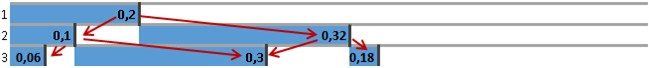
\includegraphics[scale=.85]{sections/images/imposition_of_binomial_expansion.jpg}
\floatfoot{Imposição acumulativa aos momentos lógicos descendentes.}%\footnotemark}
\end{figure}
%\footnotetext{Fonte: note}

No triângulo de pascal, Figura \ref{fig:pascal_triangle}, cada número é os dois números acima mais próximos somados. Esse número representa quantos diferentes possíveis caminhos levam até ele. Por exemplo, o número [4], na Figura \ref{fig:pascal_triangle}, representa os quatro diferentes caminhos que levam até ele. Um outro aspecto interessante do triângulo de pascal é a sequência de Fibonacci, Figura \ref{fig:pascal_triangle_fibonacci} \cite{mathisfun_pascal_triangle}.  

\begin{figure}[H]
\centering
	\begin{subfigure}[H]{0.47\linewidth}
	\centering
	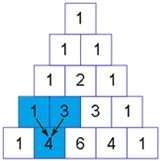
\includegraphics[width=.55\linewidth]{sections/images/pascal_triangle.jpg}
	\caption{}
	\label{fig:pascal_triangle}
	\end{subfigure}
\hfill
	\begin{subfigure}[H]{0.47\linewidth}
	\centering
	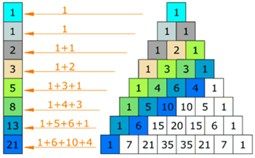
\includegraphics[width=.9\linewidth]{sections/images/pascal_triangle_fibonacci.jpg}
	\caption{}
	\label{fig:pascal_triangle_fibonacci}
	\end{subfigure}%
\caption{Características do triângulo de Pascal}

\floatfoot{Fonte: MathsIsFun, 2019.\protect\footnotemark}
\end{figure}
\footnotetext{\url{www.mathsisfun.com/pascal-triangle.html}}